\chapter{Superconductividad}

\section{Cuantización macroscópica y superconductividad}

Uno de los mayores principios de la mecánica cuántica es el hecho de que cantidades fisicas como la energía o el momentum están, bajo ciertas condiciones, cuantizados. Es decir, que sólo tienen valores discretos. Sin embargo, por un largo tiempo se creyó que la cuantización sólo era relevante para sistemas microscópicos, como los nucleos, los átomos o las moléculas. De hecho, considerando el comportamiento de objetos macroscópicos que consistan de una gran cantidad de átomos, los efectos de la cuantización no pueden ser observados, aunque cada átomo individual obedezca las leyes de la mecánica cuánica. Esto se debe al hecho de que los movimientos térmicos enmascaran las regularidades cuánticas. Sin embargo, para ciertos fénomenos ha sido demostrado que es posible observar cuantización macroscópica. Así que podemos observar la cuantización de parámetros que caracterizan a sistemas macroscópicos muchos órdenes de magnitud más grandes que sistemas como los átomos. Esto se debe a altos niveles de correlaciones por efectos de coherencia \cite{gross}.

Uno de los efectos más espectaculares de la física del estado sólido es el efecto superconductor. La superconductividad produce efectos cuánticos macroscópicos, siendo un campo perfecto para estudiar aspectos básicos en la física cuántica.

En 1911 Kamerlingh Onnes \cite{onnes} descubre que el Hg conduce sin resistencia cuando se enfría a temperatura del He líquido (4.2 K). Kamerlingh Onnes fue el primer físico que licuó el He, poco tiempo después de esto, midiendo resistividades de distintos metales a estas bajas temperaturas, se encontró, en su laboratorio, que el Hg a 4.2K conduce sin resistencia. No con una resistencia despreciablemente pequeña, sino con resistencia cero.

Una primera característica de la superconductividad es la nula resistividad por debajo de una cierta temperatura, llamada temperatura crítica.

Podría pensarse que el caso del Hg es la excepción y la cuantización macroscópica es un fenómeno particular de este elemento, sin embargo resulta que el número de elementos y materiales superconductores es muy grande. La tabla periódica está llena de elementos que, bajo cierta temperatura crítica, se convierten en superconductores. En realidad la pregunta no sería por que un elemento es superconductor, sino por qué no lo es. Ahora bien, las temperaturas a las cuales ocurre el efecto son extraordinariamente bajas. La mayoría de los superconductores tienen temperaturas críticas por debajo de los 30K y requieren ser enfriados con He líquido, lo cual quiere decir que el efecto es muy débil. Cabe mencionar que existen superconductores de ``alta temperatura'' con temperaturas críticas en el orden de los 100K y que pueden ser enfriados con N líquido, hechos a partir de cerámicas con estructuras cristalinas. El record de la mayor temperatura crítica reportada de un superconductor es -70°C \cite{drozdov}. Sin embargo, en este capítulo no haremos ninguna referencia a ellos, ya que requieren el desarrollo de teorías más avanzadas.

Ahora bien, un superconductor es mucho más que un conductor perfecto. En 1913 [ref] se comprobó que si se aplica un campo magnético exterior al material en estado superconductor, se terminaba por destruir el estado de conducción perfecta. Este campo, cuyo valor depende de la temperatura, se llama campo crítico. Tenemos así el primer indicio de que la interacción superconductividad-magnetismo juega un papel primordial en los fenómenos superconductores.

La siguiente característica fundamental de un superconductor consiste en que cuando el campo magnético aplicado no es mayor que el campo  crítico un superconductor actúa como un diamagnético perfecto ($\chi = -1$). Por lo tanto, no existen líneas de campo magnético en el interior de un material superconductor, salvo en una pequeña zona próxima a la superficie. Este efecto se conoce con el nombre de efecto Meißner-Ochsenfeld. Es importante mencionar que este no es el caso en un conductor ideal, pues en ellos el campo magnético quedaría atrapado en el material sin que haya razón para que sea expulsado.

Así la segunda característica del efecto superconductor es el diamagnetismo perfecto (efecto Meißner).

Otra característica típica de la superconductividad es que el flujo del campo magnético que atraviesa un anillo superconductor está cuantizado. Es decir, el flujo que atraviesa un superconductor vale un número entero de veces una unidad de flujo elemental llamada el fluxoide $\Phi_0$ y cuyo valor es $\Phi_0 = h /2 e$, donde $h$ es la constante de Planck y e la carga del electrón.

Por lo tanto, la tercera característica de la superconductividad es que el flujo magnético qu eatravieas un superconductor está cuantizado.

Existe otro efecto cuántico macroscópico asociado a la superconductividad, conocido como el efecto Josephson, el cuál será el fundamento de los qubits superconductores. Este efecto es un caso del efecto túnel. Si se separan dos superconductores distintos, o bien el mismo superconductor por una barrera, por ejemplo un aislante o un estrechamiento en el superconductor (lo que se conoce como una unión débil), se tiene paso de corriente por la barrera sin que aparezca caída de potencial a ambos lados de la barrera.

La cuarta característica de la superconductividad es el efecto Josephson, esto es, la existencia de un efecto túnel superconductor.

%%%%%%% Organizar estas características en una lista

\section{La teoría BCS}

En 1957 John Bardeen, Leon Cooper y J. Robert Schieffer \cite{bcs} encontraron la llave para poder explicar, desde un punto de vista microscópico, la superconductividad. Realmente existen bastantes materiales que se desvian de la teoría estricta BCS, como pueden ser aleaciones, compuestos y algunos elementos (el mismo Hg, donde se descubrió la superconductividad, es un ejemplo de superconductor que no cumple los estrictos requisitos de la teoría BCS). Esto no significa que la teoría sea incorrecta, sino incompleta y para tratar ciertas situaciones y ciertos compuestos o elementos hay que evitar algunas de las aproximaciones que se realizan en el desarrollo de esta teoría.

Experimentalmente se observó que la temperatura crítica $T_c$ de los superconductores, como el Hg, depende de la masa de los iones en el metal. Dado que existen varios isótopos del Hg se pudieron preparar varias muestras y se comprobó experimentalmente que si $M$ es la masa del ion se tiene que $T_c \propto M^{-\alpha}$ donde el exponente $\alpha$ es dependiente del tipo del metal. Esto indica que los iones de la red juegan un papel fundamental en la superconductividad. Este fenómeno se llama efecto isotópico.

Adicionalmente, existen las siguientes diferencias entre los metales normales y los superconductores:

\begin{enumerate}
\item Metal normal:
\begin{enumerate}
    \item El calor específico electrónico de un metal no superconductor a muy baja temperatura varía linealmente con la temperatura. En un metal existen dos contribuciones al calor específico, una de ellas es la normal de la red. Esta contribución varía como $T^3$ y prácticamente desaparece a bajas temperaturas. Exite otra contribución al calor específico propia de los metales. A esta contribución, que es la predominante a bajas temperaturas, es a la que nos referimos y varía como $T$.
    \item Un metal en estado normla no es transparente a la radiación visible e infrarroja.
\end{enumerate}
\item Superconductor:
\begin{enumerate}
    \item La variación del calor específico en función de la temperatura sigue una ley exponencial.
    \item En un metal en estado superconductor existe, en el rango del infrarrojo lejano, una frecuencia de corte para la cual el metal es transparente a esa radiación.
\end{enumerate}
\end{enumerate}

Estos dos efectos en superconductores son una señal de que en un superconductor existe una zanja prohibida de energía, que, como veremos en su momento, no es del mismo tipo que la que existe en semiconductores. Otra comprobación experimental de este hecho son las anomalías en el efecto túnel, conocido como túnel Giaver.

Por lo tanto, simplificando, cualquier teoría microscópica de la superconductividad tiene que dar cuenta de:

\begin{enumerate}
    \item Conductividad infinita.
    \item Intervención de la masa de iones en los fonones (vibraciones de la red cristalina).
    \item Existencia de una zanja de energía en la banda de conduccion.
\end{enumerate}

A partir de ahora solamente vamos a concentrarnos en descubrir la posible interacción responsable de que un metal conduzca sin resistencia eléctrica por debajo de un acierta temperatura.

Los electrones de conducción, por su movimiento al azar en una red cristalina, donde los iones están vibrando (fonones), cambian constantemente de momentum. La interacción electrón-fonón es la que produce la resistividad. Que un metal conduzca sin resistencia eléctrica querrá decir que los electrones de conducción en su movimiento en el cristal no cambian de momentum.

Se trata por lo tanto de encontrar una interacción en los electrones de conducción que produzca este efecto. En un cristal contamos aparentemente con pocos recursos, por un lado enemos electrones de conducción e iones que forman la red cristalina y que están fibrando, de otra forma con electrones y fonones y con una interacción fundamental entre estas cargas eléctricas, que es la interacción coulombiana. Pues bien, esto es todo lo necesario para construir la teoría BCS: electrones, fonones e interacción coulombiana.

La interaccion coulombiana electrón de conducción-red cristalina (iones) se puede ver esquemáticmanete de la siguiente forma. Supongamos un electrón de conducción que se mueve por el cristal y fijémonos en un punto concreto de la red, formada por iones positivos. Al pasar el electrón por ese punto la red, por interacción coulombiana, se sentirá atraido por ese electrón y se deformará localmente. Ya que las frecuencias de vibración de la red (de los fonones) son del orden de $10^{13} Hz$ y las velocidades de los electrones de conducción son del orden de $10^{16} Å/s$, ocurrirá que cuando la red vuelva a su posicíón de equilibrio, el electrón que la ha deformdo se encontrará muy lejos, del orden de $10^3 Å$, esto es del orden de varios cientos de parámetros de la red del ion que ha sido sacado de su posición de equilibiro. Esto es así porque las velocidades de los electrones de conducción en su movimeinto al azar, velocidades de Fermi, son muy grandes comparadas con los tiempos de relajación de la red, ligados a las frecuencias de los fonones. El segundo paso en este mecanismo es muy sencillo: Mientras que la red está deformada por sus cercanías pasan muchos otros electrones de conducción, que sienten una fuerza de atracción por la red mayor, que sin ésta no estuviera deformada. En resumen, se puede establecer una cierta conexión, una cierta interacción atractiva entre los electrones de conducción vía los fonones. Esto es, un electrón de conducción deforma la red y un segundo electrón de conducción se siente atraido por esta deformación y en cierta manera ``ligado'' al primer electrón, el cual puede estar físicamente muy alejado del primero. Esta idea de como una interacción de corto alcance electrón-fonón, puede dar lugar a una interacción de largo alcance electrón-electrón, se debe a Fröhlich (1950) \cite{frohlich} y es la base de la teoría de la superconductividad.

Ahora veamos el papel que juega la interacción coulombiana repulsiva directa entre los electrones de coonducción. Esta interacción decrece con $1/r^2$, siendo $r$ la distancia entre los electrones, es decir que disminuye rápidamente con la distancia. Luego se tendrá que la interacción neta entre los electones de conducción sera la suma de estas dos interacciones una repulvisa, que es la que podríamos decir normal y otra, vía fonón, que es atractiva. La interacción neta será atractiva solamente cuando estemos haciendo el balance entre electrones cuya interacción coulombiana repulsiva es muy pequeña, debido a la gran separación que hay entre los electrones.

Luego, Cooper demostró que si se tienen dos electones con una interacción atractiva neta, por muy pequeña que sea, el mar de Fermi de los electrones de conducción es inestrable y se produce un estado ligado con momenta $k$ y espines opuestos, llamado par de Cooper. Bardeen, Cooper y Schieffer escribieron un hamiltoniano y el estado fundamental formado por estos pares, de tal manera fueron capaces de desarrollar expresiones para la temperatura crítica superconductora; dedujeron la existencia de una zanja de energía en los superconductores, tal que para romper un par de Cooper via la interacción con los fonones de la red, hay que suministrar una energía superior o igual a la de esa zanja, y asimismo deducen el efecto isotópico.

Queda, por último, ver de dónde se obtiene la conducción eléctrica sin resistencia, es decir sin que los electrones de conducción cambien de momentum. Hay que señalar que el estado fundamental propuesto por la teoria BCS no está formado por un conunto de pares de Cooper cualesquiera. Los pares no actúan independientemente unos de otros y para romper un par hay que suministrar energía (la correspondiente a la zanja) de tipo térmico, subiendo la temperatura, o bien de tipo magnético, aplicando un campo magnético, etc. Mientras que no se suministre una energía superior a la de la zanja los electrones superconductores forman pares de Cooper de momentum constante. Esto es, conducen sin resistencia a no ser que se rompan los pares. Ahora bien, estos electrones se están moviendo en un sólido, en una red cristalina, que estará a una cierta temperatura, por debajo de la temperatura crítica, que no es suficiente para romper los pares. Por lo tanto, verán fonones e interaccionarán con ellos. ¿Cómo es posible que un electrón de una par que interacciona con un fonón (de energía menor de la necesaria para romper el par) no cambie su momentum? Esto es debido a que los pares están interrelacionados y el resto se acomoda para hacer posible que en su conjunto de $k$ no varíe. Aquí se puede utilizar una imagen debida a Schieffer. Supongamos que tenemos un conjunto de esquiadores, la mitad hombres y la mitad mujeres, que bajan una pendiente cogidos de la mano, hombre con mujer (aquí tenemos los pares de Cooper), pero estas parejas no bajan cada uno por su lado, sino que lo hacen al mismo tiempo y de alguna manera enlazados, de tal manera que si algún miembro de la pareja se encuentra en el camino un obstáculo (un fonón), siempre que no sea muy importante (de energía menor que la de la zanja) el conjunto de pares aguantarán el golpe y harán posible que se siga bajando sin perder velocidad, sin cambiar $k$, sin resistencia.

Esta interacción se puede representar con el diagrama de Feynman de la figura \ref{fig:feynmanefe}. Cuando el primer electrón llega a un punto de la red y la atrae, emite un fonón. El segundo electrón absorbe este fonón y queda acoplado al primer electrón.

\begin{figure}[H]
    \center
    \begin{tikzpicture}
      \begin{feynman}
        \vertex (a);
        \vertex [below left=of a] (i1);
        \vertex [above left=of a] (i2);
        \vertex [right=of a] (b);
        \vertex [above right=of b] (f1);
        \vertex [below right=of b] (f2);
     
        \diagram* {
          (i1) -- [fermion, edge label'=\(k\)] (a) -- [fermion, edge label'=\(k-q\)] (i2),
          (a) -- [boson, edge label'=\(q\)] (b),
          (f1) -- [fermion, edge label'=\(k\)] (b) -- [fermion, edge label'=\(k+q\)] (f2),
        };
      \end{feynman}
    \end{tikzpicture}
    \caption{Diagrama de Feynman de la interacción electrón-fonón-electrón}
    \label{fig:feynmanefe}
\end{figure}

Los electrones que participan en esta interacción son los de la banda de conducción, con energías del orden de unos pocos electrón voltio. Los fonones disponibles tienen unas energías que son como máximo del orden de \color{red}la energía de Debye\color{black}. Dado que la temperatura de Debye suele ser del orden de algo más de 100K, se tiene que las energías de los fonones disponibles son de unos pocos milielectrón voltio, esto es muy pequeña comparada con la de los electrones. se tiene que la capa de los electrones de conducción en la esfera de Fermi que intercambian fonones, según este esquema es una franja muy estrecha.

Si llamamos $\hbar k, \hbar k^\prime$ y $\hbar k_1, \hbar k_1^\prime$, los momenta de los electrones antes y después de la interacción la ley de conservación del momentum nos dice que

\begin{equation*}
    \hbar k_1 + \hbar k_1^\prime = \hbar k + \hbar k^\prime = \hbar K
\end{equation*}

donde hemos llamado $K$ al momentum del centro de masas de los electrones. Conviene aprovechar este punto para indicar el convenio habitual en cuanto al signo de la energía de los electrones. Se toman como energías positivas los valores de la energía superiores a la energía de Fermi y como energías negativas los valores inferiores a la energía, $E_F$, de Fermi. Es decir que $\epsilon_k$ será negativa si $k$ está dentro de la superficie de Fermi y positiva en caso contrario. Está claro que los únicos electrones que pueden intervernir en todo este proceso son los que tienen energías próximas a la de Fermi dado que solamente estos electrones pueden tener estados libres accesibles sin violar el principio de exclusión de Pauli. Por lo tanto, estamos solamente considerando como candidatos a electrones superconductores unos pocos de todos los de la esfera de electrones de conducción de Fermi, aquellos que están en una estrecha franja d espesor $\hbar \omega_D$ donde $\omega_D$ es la frecuencia de Debye, por lo tanto del orden de unos pocos meV de la energía de Fermi. En esta situación se conserva el momentum $\hbar K$ del centro de masas de los dos electrones. En la figura \ref{fig:goodcooper} se representa gráficamente todo lo que acabamos de decir, además se observa en esta figura que son, dentro de la estrecha franja, muy pocos los electrones que cumplen todas las condiciones y que por lo tanot pueden ser candidatos a formar pares de Cooper. Solamente los electrones cuyos momenta caen en la intersección de las dos capas esféricas son los posibles electrons superconductores. Es fácil ver que si disminuimos el valro del momentum del centro de masas del sistema la intersección aumentará y se hará máxima si hacemos $K = 0$, donde toda la franja está formada por posibles pares de Cooper. Es decir los pares de Cooper se forman con electrones de momenta opuestos, como ya habíamos anicipado unas líneas más arriba, esto es $k, -k$.  Además, este argumento que acabamos de desarrollar está apoyado en que la energía del sistema disminuye al ir formándose pares, lo que e puede demostrar, pero no de un a manera fácil.

\begin{figure}[H]
\centering 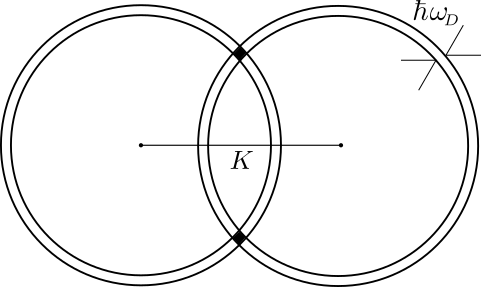
\includegraphics[width=0.6\linewidth]{img/goodcooper.png}
\caption{Construcción geométrica de los posibles electrones candidatos para formar pares de Cooper, siendo $\hbar K$ el momentum del centro de masas.}
\label{fig:goodcooper}
\end{figure}

Otro aspecto de los señalados anteriormente, que podemos abordar ahora, es que los pares estaban formados por electrones no sólo con momenta opuestos, sino también con espines opuestos, esta última característica es ahora muy fácil de tratar, dado que los electrones son fermiones, es decir cumplen el principio de exclusión de Pauli y tienen funciones de onda antisimétricas. Se puede demostrar que la parte orbital (es decir olvidándose de la parte de espín) de la función de onda de los pares de Cooper, depende tan sólo del módulo del momentum. Por lo tanto, frente al intercambio de la posicón de los dos electrones del par se tienen una función simétrica. Luego la parte de espín debe ser antisimétrica, es decir los espines de la pareja son opuestos. Se tiene que un par de Cooper esta formado por dos electrones tal que $k \uparrow, -k \downarrow$.

En este punto surge uno de los peligros típicos de la teoría BCS, que pone de manifiesto la gran cantidad de sutilezas que encierra. Dado que un par de Cooper es una entidad cuyo espin es cero, como los bosones, es fácil caer en la tentación de tratar a los pares de Cooper como bosones. Además hemos indicado que un número creciente de pares de Cooper es energéticamente favorable. Ahora bien, el principio de Pauli sigue vigente: Así, el estado formado, por ejemplo, por $k \uparrow, -k \downarrow$ no puede estar ocupado por más de un par de electrones al mismo tiempo. Además, los operadores con los que se construye el hamiltoniano de la teoría BCS, no siguen las reglas de conmutación de los operadores de bosones. Resulta de todas formas llamativo y conviene resaltarlo que la electrodinámica bosónica reproduce muy bien el comportamiento superconductor, por ejemplo la teoría clásica de la superconductividad de London se puede deducir de un gas cargado de bosones y de allí se puede extraer de una manera natural el efecto Meißner.

Pasaremos a continuación a describir de la manera más sencilla posible la función de onda del estado fundamental superconductor y algunas de las expresiones de la teoría BCS.

La función de onda del estado fundamental de $N$ electrones, según la propone la teoría BCS, es el producto de funciones de onda de pares convenientemente antisimetrizadas, que se puede representar por:

\begin{equation}
    \phi(1,2,...,N) \propto \phi(1,2)\phi(3,4)...\phi(N-1,N)
\end{equation}

Si no escribimos explícitamente la parte de espín y sólo lo hacemos con la parte orbital tendríamos

\begin{equation}
    \phi(1,2,...,N) \propto \sum_{k_1} \sum_{k_2} ... \sum_{k_3} g_{k_1} ... g_{k_{N/2}} e^{i (k_1 r_1 - r_2 k_2 + ... + k_{N/2} r_{N-1} - k_{N/2} r_N)}
\end{equation}

Donde cada término de esta función de onde describe una configuración donde los N electrones se agrupan en $N/2$ pares que son

\begin{equation}
    (k_1, -k_1) ... (k_{N/2}, -k_{N/2})
\end{equation}

La parte de espín es inmediata cada electrón de cada par tiene espines opuestos. Como vemos la funcion de onda es una función complicada que abarca todos los pares relacionados entre ellos. También se puede escribir de una manera más compacta como:

\begin{equation}
    \phi = \prod\limits_k \phi_k
\end{equation}

Antes de continuar merece la pena señalar algún otro aspecto de los pares de Cooper, estos pares están fuertemente relacionados entre sí, de tal manera que se puede decir que del orden de un millón de parestienen sus centros de masa dentro del espacio en el que se extiende un par dado, esto es los pares de electrones que forman un par de Cooer están muy alejados uno del otro, estando fuertemente correlacionados unos pares con otros. Se puede demostrar, que la disminución de la energía en la fase superconductora respecto al estado normal, debida a la interacción entre pares, depende de cómo se elijan esos pares. El conjunto de pares de Cooper no son independientes unos d eotros, están muy correlacionados.

Otro punto que hay que aclarar en lo anterior es que estamos considerando el caso en que no tenemos corriente eléctrica neta, ya que los electrones apareados tienen momentum toal cero. Los estados portadores  decorriente superconductora son aquellos en que los pares tienen momenta que serán $(k + \frac{q}{2} \uparrow, -k + \frac{q}{2} \downarrow)$ y los electrones tendrán una velocidad de arrastre neta que será

\begin{equation}
    v_a = \frac{\hbar q}{2m}
\end{equation}

Otro aspecto importante de la teoria BSC es que predice la existencia de una zanja de energía $\Delta$, zanja que se puede medir experimenalmente y que está relacionada con la temperatura crítica por la ecuación BCS. Este parámetro $\Delta$ es el parámetro crucial de la teoría BCS de que acompaña la aparición del esado superconductor.

Hay que resaltar que esta zanja reúne unas características muy particulares, por lo pronto se diferencia claramente de las zanjas que juen un papel importnate en sólidos, especialmente en los semiconductores. En superconductores tenemos una zanja que está situada en la banda de conducción y que tiene una marcada dependencia con la temperatura. Asimismo, mientras que en un semiconductor se necesita excitar por encima de la zanja a los electrones para tener conducción eléctrica, en un superconductor se tiene la supercorriente sin necesidad de tener estados excitados, se tiene conducción eléctrica por debajo del nivel de Fermi, esto es por debajo de la zanja que existe en la banda de conducción.

Este parámetro $\Delta$ aparece en la sencilla e importante relación que se obtiene en la teoría BCS

\begin{equation}
    2 \Delta(0) = 3.52 k_B T_c
\end{equation}

Donde $T_c$ es la temperatura crítica superconductora.

\section{Cuantización del flujo magnético y efecto tunel Giaver}

En la teoría de Ginzburg-Landau \cite{cyrot} de las transiciones de fase se introduce el concepto de parámetro de orden, que es una magnitud que aparece acompañando a la transición. Un ejemplo típico de parámetro de orden es la imanación de saturación, que es la magnitud que aparece cuando se tiene la transición de fase del estado paramagnético al ferromagnético. El modelo macroscópico de la superconductividad está basado en la hipótesis de que existe una función de onda macroscópica $\psi(r,t)$ que describe el comportamiento del ensemble completo de electrones superconductores y que es el parámetro de orden de la transición superconductora, tal que su módulo al cuadrado nos da la densidad de electrones superconductores que aparecen al pasar el metal del estado normal al superconductor. En el estado normal, el parámetro de orden (densidad de electrones superconductores) se desvanece. Por supuesto, esta hipótesis puede ser justificada por la teoría microscópica de la superconductividad (Teoría BCS). Esta teoría se basa en la idea de que en metales superconductores existe una fuerza atractiva entre los electrones cercanos al nivel de Fermi. A temperaturas bajo la temperatura crítica $T_c$, esta fuerza atractiva crea un nuevo estado cuántico diferente del mar de Fermi de un metal normal. Una pequeña porción de los electrones cercanos el nivel de Fermi están ligados a pares de Cooper. En el caso más simple, el movimiento interno de los pares no tiene momentum angular orbital (estado s simétrico) y consecuentemente el principio de Pauli requiere que los dos espines sean opuestos. Contrario a ligar dos átomos a una molécula, el estado orbital del par de Cooper tiene un radio mucho mayor, típicamente entre 10nm y 1$\mu$m, de manera que pares individuales se sobrelapan fuertemente en espacio y por lo tanto, la ligadura resulta cooperativa. En particular, la energía de ligadura de cualquier par depende de cuantos otros pares se hayan condensado y, más aún, el movimiento del centro de masas de los pares está fuertemente correlacionado tal que cada par reside en el mismo estado con el mismo movimiento de centro de masas. Es este estado el que describimos con una función de onda macroscópica y que le da al sistema sus propiedades superfluídicas. Por ejemplo, el movimiento del centro de masas puede ser descrito por la función de onda

\begin{equation}
    \psi(r,t) = \psi_0 e^{i \theta(r,t)} = \psi_0 e^{i k_s \dot r - i \omega t}
\end{equation}

Donde cada par tiene el mismo momentum $\hbar k_s$ o velocidad de par $v_s = \hbar k/m$. Además, se cumple que

\begin{equation}
    n_s = \abs{\psi}^2
\end{equation}
    
Donde $n_s$ es la densidad de electrones superconductores.

Por otro lado, sabemos que la cantidad de movimiento de una partícula de masa $m^*$ y carga $e^*$ en presencia de un campo magnético representado por su potencial vectorial $A$, se escribe como

\begin{equation}
    \mathbf{p} = -i \hbar \nabla \psi(r,t) = \hbar \nabla \phi = m^* \mathbf{v} + \frac{e^*}{c} \mathbf{A}
\end{equation}

Si tenemos una densidad de partículas, todas ellas teniendo el mismo momentum $\mathbf{p}$ podemos escribir $n_s \mathbf{p} = n_s (m^* \mathbf{v} + \frac{e^*}{c} \mathbf{A})$.

Recordando la expresión general de la densidad de corriente eléctrica en función de la densidad de portadores, de la carga y de la velocidad promedio se pueden escribir

\begin{equation}
    \mathbf{J} = n_s e^* \mathbf{v}
\end{equation}

Que en nuestro caso será

\begin{equation}
    \hbar \nabla \phi = \frac{m^*}{n_s e^*} J + \frac{e^*}{c} A
\end{equation}

Con esta expresión estamos preparados para demostrar la cuantización del flujo magnético en superconductores, para ellos basta con recordar algo trivial, como es que el parámetro de orden superconductor sólo puede tener un único valro en cada punto, es decir, la densidad de electrones superconductores debe ser única en cada punto, esta simple consideración se materializa en que podemos escribir

\begin{equation}
    \phi(2\pi) - \phi(0) = n 2 \pi
\end{equation}

Recordando la definición de circulación y de gradiente, y siendo $C$ un camino cerrado, la expresión anterior la podemos escribir como

\begin{equation}
    \oint\limits_C \nabla \phi dl = n 2 \pi
\end{equation}

Si ahora suponemos que este camino $C$ está en el interior de un superconductor, alejado de los bordes y rodeando a un hueco, como se representa en la figura \ref{fig:fluxquant} y suponemos que tenemos aplicado un campo magnético a este superconductor, se tiene

\begin{equation}
    \oint\limits_C (\frac{m^*}{\hbar n_s e^*} J + \frac{e^*}{\hbar e} A) dl = n 2 \pi
\end{equation}

\begin{figure}[H]
\centering 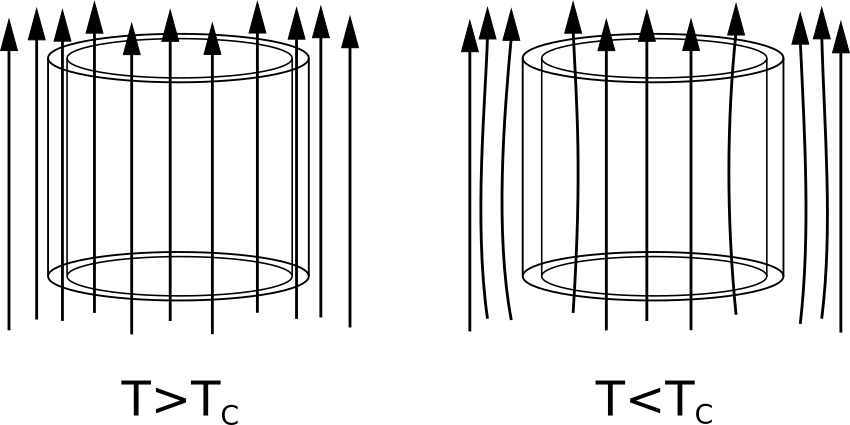
\includegraphics[width=0.8\linewidth]{img/fluxquant.png}
\caption{Cuantización del flujo magnético}
\label{fig:fluxquant}
\end{figure}

Dado que estamos en un camino interior al superconductor y allí no existe corriente (las únicas corrientes que existen en una situación como la que estamos describiendo, están apantallando el campo magnético y están situadas cerca de los bordes tanto de la cavidad como de la superficie del material superconductor), tendremos

\begin{equation}
    \oint A dl = \frac{n h c}{e^*}
\end{equation}

Recordando el teorema de Stokes se tiene

\begin{equation}
    \oint\limits_C A dl = \iint\limits_S B ds = \Phi
\end{equation}

Que en nuestro caso será $\Phi = n \Phi_0$ expresión que nos indica que el flujo magnético que encierra la cavidad es un número entero de un flujo elemental conocido con el nombre de fluxoide y cuyo valor es

\begin{equation}
    \Phi_0 = \frac{h c}{2 e} = 2.07 10^{-7} gauss\ cm^2
\end{equation}

Siendo $e^*$ la carga del portador de corriente, el par de Cooper $e^* = 2e$.

Este efecto fue encontrado experimentalmente de forma simultánea en 1961 por Deaver-Fairbanks \cite{deaver} y por Doll-Näbauer [ref].

El efecto túnel es un efecto típico del carácter cuántico de los electrones, desde el punto de vista de la física clásica es completamente imposible que se produzca el efecto que vamos a discutir.

Los electrones se pueden representar por funciones de onda, de tal manera que existe una cierta probabilidad de que un electrón pueda ir de un metal a otro atravesando una barrera aislante estrecha, que puede ser vacío o un óxido. La función de onda del electrón decae de una manera exponencial fuera de la superficie del metal, la amplitud de la onda no es totalmetne nula fuera del metal, es como si el electrón se desparramase fuera de la superficie. Si situamos un metal junto al otro, separados tan sólo por una barrera, como puede ser, por ejemplo, el óxido de la superficie, existe una probabilidad pequeña, pero no nula de que el electrón atraviese ese túnel y aparezca al otro lado, en el otro metal.

Antes de seguir hay que hacer notar que la energía necesaria para hacer pasar un electrón que está en el nivel de Fermi de un metal al vacío (función de trabajo del metal) es mayor que la energía necesaria para transferir ese electrón a un aislante.

Por razones de simplicidad vamos a hacer toda la discusión siguiente, salvo cuando se diga expresamente lo contrario, para temperatura de 0K. La figura \ref{fig:el1} nos indica la situación entre dos partes del mismo metal separadas por un aislante. Todos los estados por debajo de la energía de Fermi están ocupados, mientras que todos los estados por encima de $E_F$ están vacíos.

\begin{figure}[H]
\centering 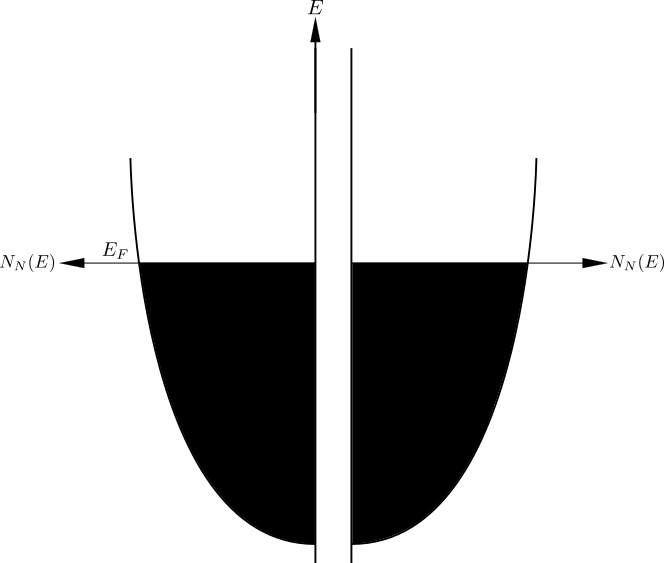
\includegraphics[width=0.8\linewidth]{img/el1.png}
\caption{Imposibilidad de efecto túnel a través de la barrera}
\label{fig:el1}
\end{figure}

Para que se pueda tener efecto túnel hacen falta dos condiciones. La primera es que, como es lógico, los electrones solamente pueden ir de un estado ocupado a un estado desocupado y la segund aes que se tiene que conservar la energía, es decir que las transiciones, en la gráfica, tienen que ser horizontales. Por lo tanto en la situación de la figura \ref{fig:el1} no tendremos efecto túnel. No se pueden tener transiciones horizontales al no existir estados vacíos. Todos los estados en el mismo nivel de energía, a ambos lados de la barrera, están ocupados.

Si aplicamos una diferencia de potencial constante a la barrera lo que estamso haciendo es aumentando la energía de los electrones de un lado de la barrera respecto al otro y entonces tenemos la posibilidad de que se tenga corriente por efecto túnel, figura \ref{fig:el2}.

\begin{figure}[H]
\centering 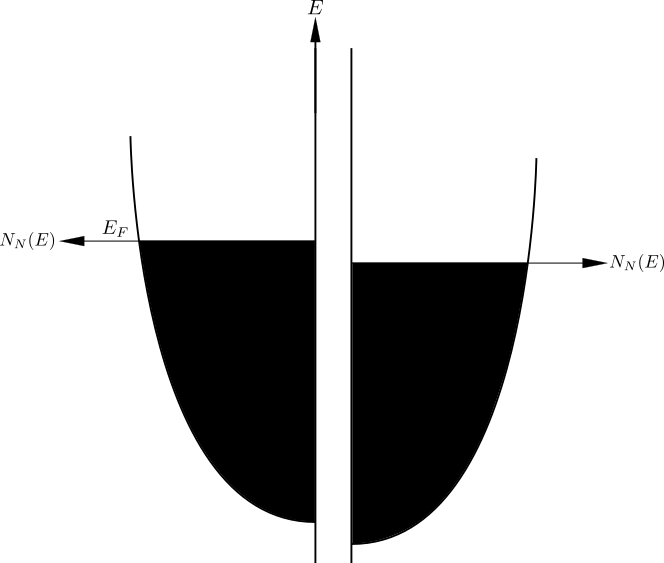
\includegraphics[width=0.8\linewidth]{img/el2.png}
\caption{Posibilidad de efecto túnel a través de la barrera}
\label{fig:el2}
\end{figure}

La intensidad de esta corriente túnel depende de varios parámetros. Por ejemplo, a mayor diferencia de potencial aplicada mayor correitne. Está claro que cuantos más estados tengamos en el nivel de Fermi mayor será la probabilidad de tener corriente túnel, lo cual puede indicar que quizáß con experimentos de efecto túnel podemos obtener información sobre este importante parámetro y en general sobre la superficie de Fermi, pero como es de esperar la corriente túnel también depende de la anchura, altura y forma de la barrera y estos parámetros son muy difíciles de determinar, lo cual hace que en metales normales del efecto túnel se obtenga una información mucho menos rica de lo que se podía esperar. Ocurre todo lo contrario con el efecto túnel cuando uno de los dos metales está en estado superconductor, como pasaremos a ver a continuación.

La existencia de una zanja de energía en el estado superconductor \ref{fig:el3} hace que el efecto túnel en una estructura formada por superconductor-aislante-metal en estado normal, tenga características especiales (Giaver, 1960 [ref]). Es claro que necesitamos previamente disponer de electrones normales por encima de la zanja superconductora, esto es hay que romper pares de Cooper, como primera medida, es decir diferencias de potencial aplicadas menores que la zanja no producirán efecto túnel. Esto es, se tiene que diferencias de potencial aplicadas a la barrera no producen corriente túnel, salvo que venzan un valor umbral, qu es precisamente el ancho de la zanja. De entrada ya tenemos una muy importante propiedad del efecto túnel superconductor, que nos permite medir la zanja superconductora y medir la variación de esta zanja con la temperatura.

\begin{figure}[H]
\centering 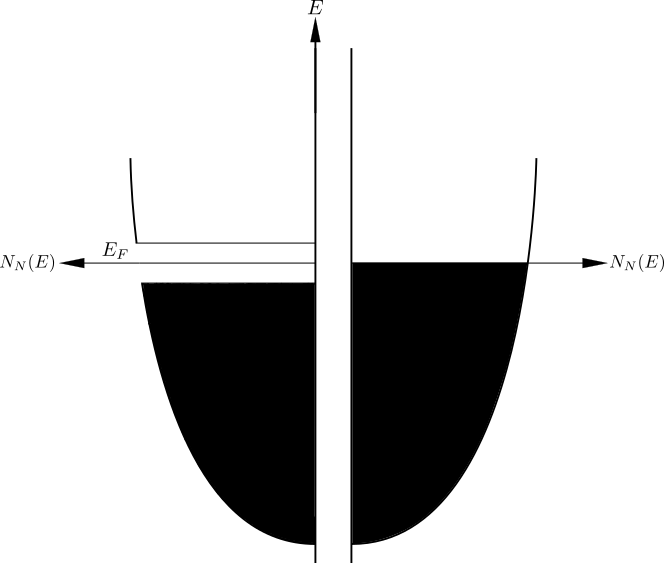
\includegraphics[width=0.8\linewidth]{img/el3.png}
\caption{Efecto Giaver: Efecto túnel entre un metal y un superconductor}
\label{fig:el3}
\end{figure}

\section{Efecto Josephson}

El efecto Josephson fue postulado teóricamente por Josephson (1962) \cite{josephson} y comprobado experimentalmente por P.W. Anderson y Rowell (1963) \cite{rowell} y por Shapiro (1963) \cite{shapiro}, casi simultáneamente. Este es un efecto túnel de pares de Cooper entre superconductores, mientras que el efecto túnel tratado en las líneas anteriores es túnel de electrones normales entre superconductores o entre un metal normal y un superconductor. En concreto la sugerencia de Josephson es que puede existir efecto túnel entre dos superconductores que se encuentren separados por una barrera aislante (en principio más delgada que las tratadas en el efecto túnel Giaver), donde la corriente túnel sea exclusivamente de pares de Cooper sin que se tenga una diferencia de potencial entre ambos lados de la barrera.

Se va a seguir la deducción de Feynman por su sencillez y claridad. Supongamos que tenemos un superconductor separado en dos partes por un aislante lo suficientemente estrecho como para que la función de onda superconductora a un lado de la barrera se sobrelape con la del otro lado. Sean $\psi_1$ y $\psi_2$ las funciones de onda superconductoras a los dos lados de la barrera (1) y (2).

El tunelamiento de pares del lado (2) al lado (1) aumenta la amplitud $\psi_1$ de la función de onda de los pares en el lado (1), es decir, aumenta la cantidad de pares de Cooper en el lado (1). Supongamos que el ritmo de crecimiento de $\psi_1$ es proporcional a $\psi_2$, amplitud de la funcion de onda de los pares en el lado (2). Podemos escribir el ritmo de cambio de $\psi_1$ de la forma $A \psi_2$ donde $A$ es una característica de la barrera y nos da información de la probabilidad de transferencia de pares del lado (2) al lado (1).

Podemos escribir la ecuación de Schrödinger para el lado superconductor (1) teniendo en cuenta esto último, como

\begin{equation}
    \frac{-\hbar}{i} \frac{\partial \psi_1}{\partial t} = E_1 \psi_1 + A \psi_2
\end{equation}

donde $E_1$ es la energía del estado más bajo de energía del superconductor del lado (1).

Análogamente, podemos escribir para el superconductor del lado (2)

\begin{equation}
    \frac{-\hbar}{i} \frac{\partial \psi_2}{\partial t} = E_2 \psi_2 + A \psi_1
\end{equation}

Escribiendo explícitamente la función de onda superconductora, $\psi_i = \sqrt{n_{s_i}} e^{i \varphi_i}$, donde, como ya vimos, $n_{s_i}$ es la densidad de electrones superconductores en el lado (i).

Por lo tanto las ecuaciones anteriores pueden ser escritas como

\begin{align}
    \frac{-\hbar}{i} \frac{1}{2 \sqrt{n_{s_1}}} \frac{\partial n_{s_1}}{\partial t} + \hbar \frac{\partial \varphi_1}{\partial t} \sqrt{n_{s_1}} &= E_1 \sqrt{n_{s_1}} + A \sqrt{n_{s_2}} e^{i (\varphi_2 - \varphi_1)} \\
    \frac{-\hbar}{i} \frac{1}{2 \sqrt{n_{s_2}}} \frac{\partial n_{s_2}}{\partial t} + \hbar \frac{\partial \varphi_2}{\partial t} \sqrt{n_{s_2}} &= E_2 \sqrt{n_{s_2}} + A \sqrt{n_{s_1}} e^{i (\varphi_1 - \varphi_2)}
\end{align}


Si ahora igualamos las partes reales y las partes imaginarias de estas ecuaciones tenemos

\begin{align}
    \frac{\partial \varphi_1}{\partial t} &= \frac{j_0}{2 n_{s_1}} \cos(\delta) + E_1/\hbar \\
    \frac{\partial \varphi_2}{\partial t} &= \frac{j_0}{2 n_{s_2}} \cos(\delta) + E_2/\hbar \\
    \frac{\partial n_{s_1}}{\partial t} &= -j_0 \sin(\delta) \\
    \frac{\partial n_{s_2}}{\partial t} &= j_0 \sin(\delta)
\end{align}

Donde $\delta = \varphi_2 - \varphi_1$ y $j_0 = \frac{2 A}{\hbar} (n_{s_1} n_{s_2})^{\sfrac{1}{2}}$. En lo que sigue, asumiremos que se tiene el mismo superconductor en ambos lados, así que tomaremos $n_{s1} = n_{s2}$. Entonces:

\begin{align}
    \frac{\partial \delta}{\partial t} &= \frac{\partial \varphi_2}{\partial t} - \frac{\partial \varphi_1}{\partial t} = (E_2 - E_1)/\hbar \\
    j &= \frac{\partial n_{s_2}}{\partial t} = - \frac{\partial n_{s_1}}{\partial t} = j_0 \sin(\delta)
\end{align}

De aquí salen directamente las relaciones de Josephson para corriente y voltaje:

\begin{align}
    V_J &= \frac{\hbar}{2e} \frac{\partial \delta}{d t} \\
    I_J &= I_0 \sin(\delta)
\end{align}

Donde el voltaje $V_J$ es la diferencia de potencial entre los dos extremos de la junción de Josephson e $I_J$ es la supercorriente que fluye a través de ésta.

Existe una clara diferencia entre este efecto túnel y el considerado al principio. En este caso de efecto Josephson tenemos túnel de pares de Cooper, mientras que en el caso anterior el túnel era de electrones individuales. En el efecto Josephson son bastante estrechas del orden o menores que la longitud coherente (tamaño de los pares de Cooper), en realidad el aislante actúa como un mal superconductor, las funciones de onda de ambos lados se pueden solapar, existiendo una difrencia de fase a ambos lados de la barrera y como resultado de todo esto se establece una corriente continua a través de la barrera. En ralidad, se puede demostrar que el mínimo de enrgía se alcanza cuando las fases se igualan y por lo tanto no se tiene correitne a través de la barrera, pero basta con aplicar una correinte de una fuente externa, siempre menor que $I_0$, para que las fases dejen de ser iguales y si esta desigualdad no varía con el tiempo, se tiene a través de la barrera una correitne constante sin que se tenga caída de potencial. no hace falta colocar un óxido, un aislante, para que actúe de barrera se puede utilizar un estrechamiento en el supercondcutor, producido mediante una técnica conocida como fotolitografía, o cualquier otra técnica que nos produzca que una parte del supercondutor esté unida a otra mediante un estrangulamiento lo suficientemente estrecho como para ser una unión débil. También se peuden obtener este tipo de uniones débiles con contactos entre superconductores de tipo puntual, o bien separando dos supercondcutores por una capa delgada de un metal en estado normal. Como acabamos de mencionar el tamaño de los pares de Cooper es una indicación del orden de magnitud de esta unión débil.

Los órdenes de magnitud de los parámetros que intervienen en el efecto Josephson son, para una unión de $1mm^2$ de área $R = 1 \Omega$, $I_0 = 1 mA$ y $\Delta = 1meV$. Normalmente las densidades de corriente a través de las uniones son dle orden de un millón de veces menores que las densidades de corriente crítica superconductoa en un superconductor. Es decir, en general, en un superconductor se tiene que pasar de la densidad de correinte crítica para hacer desaparecer la superconductividad, pero si el superconductor tiene en algún punto una unión débil densidades de corriente un millón de veces menores hacen que se tenga caída de potencial en el paso de correitne por la unión.

Si hacemos pasar una corriente mayor que $I_0$ aparece una diferencia de potencial y teniendo en cuenta que al mismo tiempo que este efecto túnel (Josephson) de pares podemos tener el efecto túnel normal (Giaver) de electrones, el resultado se puede ver en la figura \ref{fig:ivjj} donde se representa la curva característica I,V. Como sea la conexción en la realidad entre estos dos túneles depende de las características de l aunión y del circuito exterior.

\begin{figure}[H]
\centering 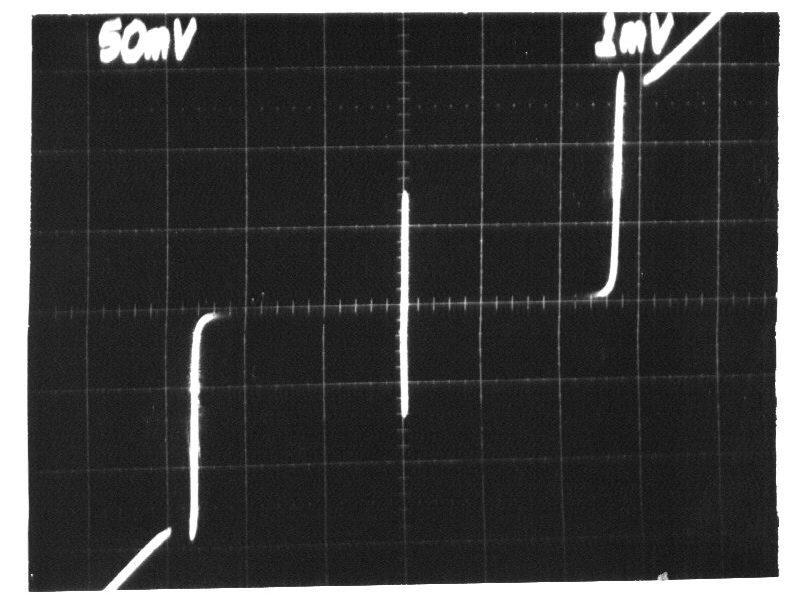
\includegraphics[width=0.8\linewidth]{img/IVJJ.JPG}
\caption{Curva característica de una unión Josephson}
\label{fig:ivjj}
\end{figure}

Finalmente hay que considerar lo que ocurre si aplicamos a la unión Josephson una diferencia de potencial externa constante, V, o lo que es lo mismo, tenemos una intensidad pasando por la barrera superor a $I_0$. El cálculo es análogo al anterior, muy sencillo y nos conduce a que la intensidad a través de la barrera tiene la expresión

\begin{equation}
    I = I_0 \sin( (\varphi_2 - \varphi_1) + \omega t) = I_o \sin(\delta + \omega t)
\end{equation}

Donde $\omega = \frac{2 eV}{\hbar}$.

En realidad el punto de partida de esta deducción es la dependencia con el tiempo de la fase, una diferencia de potencial aplicada a l aunión lo que hace es variar en el tiempo la fase y el ritmo de variación d ela fase viene dado por la ecuación $\frac{d \delta}{d t} = \frac{E_2 - E_1}{\hbar} = \frac{qV}{\hbar} = \frac{2 eV}{\hbar}$.

Es decir, una diferencia de potencial constante aplicada a una barrera Josephson produce una corriente alterna de pares (una supercorreinte), por ejemplo una diferencia de potencial del orden de $1 \mu V$ da lugar a una corriente que oscila con una frecuencia de 484MHz. Además de esta corriente de pares tenemos la correitne debida al efecto túnel normla de los electrones individuales. Ahora podemos volver a la figura \ref{fig:ivjj} donde tendremos que hasta que se alcanza el valor $I_0$ tenemos paso de correinte por la unión sin caida de potencial. una vez que $I > I_0$, entonces aparece un voltaje y nos situamos en un punto de la gráfica del efecto túnel de electrones normales (Giaver), tenemos una diferencia de potencial aplicada, luego existe túnel normal y además, esto no está represntado en la fëáfica, tenemos una supercorriente (corriente de pares de Cooper) que está oscilando.

\section{Componentes de la corriente en las junciones de Josephson}

Esta corriente tiene tres componentes:

\begin{enumerate}
    \item $I_d$, la corriente de desplazamiento: Como la corriente en un capacitor. La junción de Josephson forma un capacitor de placas parelelas superconductoras con un material aislante o un metal normal entre ellas, entonces podemos hablar de una corriente de desplazamiento $I_d$. La capacitancia $C$ de este dispositivo está definida de la misma manera que en el estado normal: $C = \epsilon_r \frac{A}{4 \pi d}$, donde $\epsilon_r$ es la constante dieléctrica relativa de la capa que separa a los dos superconductores, $d$ la separación de los superconductores y $A$ el área de los mismos.
    \item $I_n$, la correinte ordinaria: Por los electrones individuales. Cuando la temperatura $T \neq 0$, siempre habrá movimiento térmico de cargas cuya energía es del orden de $k_b T$, donde $k_B$ es la constante de Boltzmann. Cuando $T$ es menor, pero cercano a la termperatura crítica $T_c$, la energía de acoplamiento de los pares de Cooper $E_g = 2 \Delta$ es mucho menor a $k_B T$, lo cual resulta en la disminución de los pares de Cooper y el aumento de la concentración de eletrones normales. Si el voltaje a través de la junción es mayor al asociado a la energía de la brecha $V_g = \abs{\Delta_1 + \Delta_2}/e$, los pares de Cooper de un lado de la unión se rompen y uno de los electrones de cada uno de los pares disueltos pasa al otro lado, es decir, se produce un tunelamiento de electrones normales. Si la concentración de electrones individuales aumenta, el comportamiento de la unión tenderá a uno de tipo óhmico, es decir, la junción tenderá a comportarse como una resistencia.
    \item $I_s$, la supercorriente: Por los pares de Cooper. Se puede expresar en términos de una corriente crítica $I_0$ y la diferencia de fase entre las funciones de onda macroscópicas de las dos placas superconductoras, de manera que $I_s = I_0 \sin(\delta)$. La corriente crítica es un parámetro experimental importante del dispositivo que puede alterarse tanto por la temperatura como por un campo magnético aplicado.
\end{enumerate}

\section{Qubits superconductores}
Los qubits superconductores se basan en circuitos osciladores no lineales, hechos a partir de JJs \cite{wendin}.
\vspace{0.5cm}

El Hamiltoniano de un oscilador armónico LC está dado por 

\begin{equation}
\hat{H} = E_C \hat{n}^2 + E_L \frac{\hat{\phi}^2}{2},
\end{equation}

donde $\hat{n}$ es la cantidad de pares de Cooper inducidos en el capacitor (En otras parabras, la carga inducida en el capacitor, medida en unidades de $2e$), y $\hat{\phi}$ es la diferencia de fase sobre el inductor. La carga $\hat{n}$ y la fase $\hat{\phi}$ no conmutan, $\comm{\hat{\phi}}{\hat{n}}=i$, lo que significa que sus valores esperados no se pueden medir simultaneamente. $E_C=\frac{(2e)^2}{2C}$, $E_L=\frac{\hbar^2}{(2e)^2L}$ y la distancia entre niveles de energía del oscilador armónico $\hbar \omega = \frac{\hbar}{\sqrt{LC}}=\sqrt{2E_LE_C}$.
\vspace{0.5cm}

Para poder servir como qubit, el oscilador debe ser anarmónico, de manera que se pueda operar sobre un par específico de niveles de energía. Al agregar una JJ, el Hamiltoniano del circuito LCJ se convierte en:

\[
\hat{H} = E_C (\hat{n}-n_g)^2 - E_{J0} \cos( \hat{\phi} ) + E_L \frac{(\hat{\phi}-\phi_e)^2}{2},
\]

donde $n_g$ es la carga inducida por voltaje en el capacitor C (isla qubit) y $\phi_e$ es la fase inducida por flujo sobre la JJ. La energía de Josephson $E_{J0}$ está dada por $E_{J0}=\frac{\hbar}{2e}I_0$ en términos de la corriente crítica $I_0$ de la unión. Usualmente, la JJ es del tipo Superconductor-Aislante-Superconductor con corriente crítica fija.

Con el fin de introducir la inductancia no lineal de Josephson, empezamos por 

\[
I_J = I_0 \sin(\phi)
\]

Combinado con la ley de Lenz:

\[
V = \frac{d\Phi}{dt} = \frac{\Phi_0}{2\pi} \frac{d\phi}{dt}, \hspace{20pt} \Phi_0=\frac{h}{2e}
\]

Se encuentra que:

\[
V = \frac{\Phi_0}{2\pi} \frac{1}{I_0\cos(\phi)} \frac{dI_J}{dt}
\]

Definiendo $L_J = V (\frac{dI_J}{dt})^{-1}$, se obtiene finalmente la inductancia de Josephson $L_{J0}$:

\[
L_J = \frac{\Phi_0}{2\pi} \frac{1}{I_0 \cos(\phi)} = L_{J0} \frac{1}{\cos(\phi)}
\]

Esto define la inductancia de Josephson de la JJ aislada y nos permite expresar la energía de Josephson como $E_{J0} = \frac{\hbar^2}{(2e)^2L_{J0}}$

\begin{align*}
[E_C (-i\hbar \frac{\partial}{\partial\phi}-n_g)^2 + U(\phi)] \psi = E \psi \\
U(\phi) = -E_{J0} \cos(\phi) + E_L \frac{(\phi-\phi_e)^2}{2}
\end{align*}

\begin{enumerate}
\item $E_L = 0 \quad (L \sim \infty)$ :
\item $E_L \approx E_{J0}$ :
\end{enumerate}

\section{Arquetipos de qubits superconductores}

\subsection{Qubit de carga}

Si $E_L$ tiende a cero, la carga almacenada en la isla superconductora entre el capacitor y  la unión Josephson se puede usar como qubit. El potencial de este tipo de qubit es de forma de coseno.

\subsection{Qubit de flujo}

Si $E_L$ es comparable con $E_{J0}$, el flujo a través del lazo formado por el inductor y la unión Josephson se puede usar como qubit. El potencial de este tipo de qubit es de forma cuártica.

\subsection{Qubit de fase}

Si se polariza la unión Josephson con una fuente de corriente, la fase en ambos extermos de la unión Josephson se puede usar como qubit. El potencial de este tipo de qubit es de forma cúbica.

\section{Transmones}

Los transmones son un tipo de qubit de carga. Tratando el transmón como un sistema de dos niveles acoplado linealmente a un oscilador monomodo, su Hamiltoniano toma la siguiente forma:

\[
\hat{H} = \hat{H}_q + \hat{H}_{qr} + \hat{H}_r = -\frac{1}{2} \epsilon \sigma_z + g \sigma_x (a+a^\dag) + \hbar \omega (a^\dag a + \frac{1}{2})
\]

donde $\epsilon$ es la energía de excitación del qubit, $g$ es el acoplamiento qubit-oscilador y $\omega$ es la frecuencia del oscilador.
\vspace{0.5cm}

Introduciendo los operadores escalera del qubit, $\sigma_\pm = \frac{1}{2}(\sigma_x \pm i \sigma_y)$, el término de interacción $\hat{H}_{qr}$ se puede dividir en dos términos, el de Jaynes-Cummings (JC) y el anti-Jaynes-Cummings (AJC):

\[
\hat{H}_{qr} = \hat{H}_{qr}^{JC} + \hat{H}_{qr}^{AJC} = g(\sigma_+ a + \sigma_- a^\dag) + g(\sigma_+ a^\dag + \sigma_- a)
\]

Este Hamiltoniano describe el modelo cuántico canónico de Rabi (canonical quantum Rabi model - QRM). Las ecuaciones ()() son completamente generales y aplicables a cualquier sistema qubit-oscilador. Mantener sólo el término JC correponde a realizar la aproximación de onda rotativa (rotating wave approximation - RWA).

\section{Hamiltonianos multiqubit de transmones}
Omitiendo el término del oscilador, el Hamiltoniano toma la siguiente forma general:

\[
\hat{H} = \hat{H}_q + \hat{H}_{qr} + \hat{H}_{qq} = -\frac{1}{2} \sum\limits_i \epsilon_i \sigma_{zi} + \sum\limits_i g_i \sigma_{xi} (a+a^\dag) + \frac{1}{2} \sum\limits_{i,j;\nu} \lambda_{\nu,ij} \sigma_{\nu i} \sigma_{\nu j}
\]

Por simplicidad, se considera que el término $\hat{H}_{qr}$ se refiere sólo a la lectura y las operaciones de bus, dejando la interacción indirecta qubit-qubit via el resonador ser incluidas en $\hat{H}_{qq}$ via la constante de acoplamiento $\lambda_{\nu,ij}$.

\subsection{Acoplamiento capacitivo}
\begin{align*}
\hat{H}_{qq} = \lambda_{1 2} \sigma_{x1} \sigma_{x2} \\
\lambda_{1 2} = \frac{1}{2} \sqrt{E_{1 0, 1} E_{1 0, 2}} \frac{\sqrt{E_{E_{C1}} E_{E_{C2}}}}{E_{Cc}} = \frac{1}{2} \sqrt{E_{1 0, 1} E_{1 0, 2}} \frac{Cc}{\sqrt{C_1 C_2}} \approx \frac{1}{2} E_{1 0} \frac{C_c}{C} \\
\hat{H}_{qq} = \lambda_{1 2} (\sigma_{+1} \sigma_{-2}  + \sigma_{-1} \sigma_{+2})
\end{align*}

\subsection{Acoplamiento por el resonador}
\begin{align*}
\hat{H}_{qq} = \lambda_{1 2} \sigma_{x1} \sigma_{x2} \\
\lambda{1 2} = \frac{1}{2} g_1 g_2 (\frac{1}{\Delta_1} + \frac{1}{\Delta_2} \equiv g_1 g_2 \frac{1}{\Delta}) \\
\Delta_i = \epsilon_i - \hbar \omega
\end{align*}

\subsection{Acoplamiento de JJ}
\begin{align*}
\hat{H}_{qq} = \lambda_{1 2} \sigma_{y1} \sigma_{y2} \\
\lambda_{1 2} \approx \frac{1}{2} E_{1 0} \frac{L_c}{L_J} \frac{\cos(\delta_c)}{2L_c \cos(\delta_c) + L_{J c}}
\end{align*}

\subsection{Acoplamiento afinable/calibrable}

\section{Compuertas cuánticas en transmones}

\subsection{El operador de evolución temporal}
La evolución temporal de un sistema complejo (many-body) puede ser descrita por la ecuación de Schrödinger para el vector de estado $\ket{\psi(t)}$:

\[
i \hbar \frac{\partial}{\partial t} \ket{\psi(t)} = \hat{H}(t) \ket{\phi(t)}
\]

en términos del operador evolución $\hat{U}(t,t_0)$

\[
\ket{\psi(t)} = \hat{U}(t,t_0) \ket{\psi(t_0)}
\]

determinado a partir del Hamiltoniano complejo (many-body) dependiente del tiempo del sistema:

\[
\hat{H} = \hat{H}_{syst} + \hat{H}_{ctrl}(t)
\]

describiendo el sistema intrínseco y las operaciones de control aplicadas. Las compuertas son el resultado de aplicar pulsos de control específicos a partes selectas de un circuito físico. Esto afecta varios términos del Hamiltoniano, haciéndolos dependientes del tiempo.

Para el transmón, el Hamiltoniano del sistema bajo la RWA toma la forma:

\[
\hat{H}_{syst} = -\frac{1}{2} \sum\limits_{\nu i} \epsilon_i \sigma_{z i} + \sum\limits_{i} g_i (\sigma_{+ i} a + \sigma_{- i} a^\dag) + \hbar \omega a^\dag a + \frac{1}{2} \sum\limits_{i,j;\nu} \lambda_{\nu, ij} (\sigma_{+ i} \sigma_{- j} + \sigma_{- i} \sigma_{+ j})
\]

y el término de control se puede escribir como:

\[
\hat{H}_{ctrl} = \sum\limits_{i; \nu} f_{\nu i}(t) \sigma_{\nu i} + \frac{1}{2} \sum\limits_{i,j;\nu} h_{\nu, ij}(t) \sigma_{\nu i} \sigma_{\nu j} + k(t) a^\dag a
\]

\subsection{Pulsos de microondas}

$$\hat{H}_d = \sum\limits_k (a+a^\dagger) (\xi_k e^{-i\omega_d^{(k)}t} + \xi_k^*e^{i\omega_d^{(k)}t})$$

RWA: $$\hat{H}_d=\sum\limits_k a\xi_k^*e^{i\omega_d^{(k)}t}+ a^\dagger\xi_ke^{-i\omega_d^{(k)}t}$$

\subsection{Régimen rotacional del pulso}

Trabajando con un sólo modo a la vez, se aplica la siguiente transformación $U(t) = exp[-i \omega_d t(a^\dagger a + \sum\limits_i \sigma_{z i})]$ para entrar en el régimen rotacional del pulso de control.

$$\hat{H} = U^\dagger (\hat{H}_{syst} + \hat{H}_d) U - i U^\dagger \dot{U}$$
$$ \hat{H} = \Delta_c a^\dagger a + \frac{1}{2} \sum\limits_i \Delta_{qi} \sigma_{zi} + \sum\limits_i g_i (a \sigma_{+ i} + a^\dagger \sigma_{- i}) + (a\xi^*e^{i\omega_d t}+a^\dagger\xi e^{-i\omega_d t})$$

$\Delta_c = \omega_c - \omega_d \qquad \quad \Delta_{qi} = \omega_{qi} - \omega_d$

\subsection{Efecto del pulso sobre el qubit}

Luego se aplica el operador de desplazamineto $D(\alpha) = exp[\alpha a^\dagger - \alpha^* a]$ sobre el campo $a$ con $\dot{\alpha} = -i \Delta_c \alpha -i \xi e^{-i \omega_d t}$ para eliminar el efecto directo del pulso sobre la cavidad.

$$\hat{H} = D^\dagger (\alpha) \hat{H}_{old} D(\alpha) -i D^\dagger(\alpha) \dot{D}(\alpha)$$

$$\hat{H} = \Delta_c a^\dagger a + \frac{1}{2} \sum\limits_i \Delta_{qi} \sigma_{zi} + \sum\limits_i g_i (a \sigma_{+i} + a^\dagger \sigma_{-i})$$
$$ + \sum\limits_i g_i (\alpha \sigma_{+i} + \alpha^* \sigma_{-i}) - \Delta_c \alpha \alpha^* $$

El término $-\Delta_c \alpha \alpha^*$ se desprecia, ya que sólo representa una fase global en la evolución del sistema.

\subsection{Régimen dispersivo}

Finalmente, aplicamos la transformación $U = exp[\sum\limits_i \frac{g_i} {\Delta_i} (a^\dagger \sigma_{-i} - a \sigma_{+i})]$, donde $\Delta_i = \omega_{qi} - \omega_c$ y realizamos la aproximación de segundo grado sobre los términos $\frac{g_i}{\Delta_i} \ll 1$.

$$\hat{H} = U^\dagger \hat{H}_{old} U$$
$$\hat{H} \approx \tilde{\Delta}_c a^\dagger a + \frac{1}{2} \sum\limits_i \tilde{\Delta}_{qi} \sigma_{zi} + \sum\limits_i (\Omega_i \sigma_{+i} + \Omega_i^* \sigma_{-i})$$
$$+ \sum\limits_{i \neq j} \frac{g_i g_j}{2 \Delta_i} (\sigma_{-i} \sigma_{+j}+\sigma_{+i} \sigma_{-j})$$

$\tilde{\Delta}_c = (\omega_c + \sum\limits_i \chi_i \sigma_{zi}) - \omega_d
 \qquad
 \tilde{\Delta}_{qi} = (\omega_{qi} + \chi_i) - \omega_d
 \qquad
 \chi_i = \frac{g_i^2}{\Delta_i}$

\subsection{Rotaciones X-Y}

Tomando $\Omega(t) = \Omega^x(t) \cos(\omega_d t) + \Omega^y \sin(\omega_d t)$, donde $\omega_d$ es igual a la frecuencia de resonancia de uno de los qubits logramos rotaciones sobre los ejes X e Y. Las amplitudes de estas rotaciones vienen dadas por $\int_0^{t_0} \Omega^x(t) dt$ y $\int_0^{t_0} \Omega^y(t) dt$, respectivamente, donde $t_0$ es la duración del pulso.

$$\hat{H} \approx \tilde{\Delta}_c a^\dagger a + \frac{1}{2} \tilde{\Delta}_q \sigma_z + \frac{1}{2} (\Omega^x(t) \sigma_x + \Omega^y(t) \sigma_y)$$

\subsection{Compuerta de entrelazamiento}

Ejemplo con sólo dos qubits

$$\hat{H} \approx \frac{1}{2} \tilde{\Delta}_{q_1} \sigma_{z_1} + \frac{1}{2} \tilde{\Delta}_{q_2} \sigma_{z_2} + \frac{g_1 g_2 (\Delta_1 + \Delta_2)}{2 \Delta_1 \Delta_2} (\sigma_{-_1} \sigma_{+_2} + \sigma_{+_1} \sigma_{-_2})$$

Variando la frecuencia de resonacia de los qubit, se puede variar el acoplamiento entre estos. 

\subsection{Compuertas compuestas}

Con los transmones se pueden realizar rotaciones X-Y y la compuerta iSWAP. Sin embargo, los algoritmos no se escriben en función de sólo estas compuertas, también se necesitan H, CNOT, entre otras. Entonces, debemos construir estas otras compuertas en función de Rx, Ry e iSWAP. Esto es posible, ya que con secuencias de rotaciones en X e Y se puede realizar cualquier compuerta de un sólo qubit, ya que estas consisten de rotaciones en la esfera de Bloch y con rotaciones sobre dos ejes ortogonales se pueden lograr rotaciones sobre cualquier eje en la esfera. Luego, con un set universal de compuertas de un sólo qubit y una compuerta de entrelazamiento, se tiene un conjunto universal de compuertas cuánticas.

Las otras compuertas que necesitaremos, se construyen de la siguiente manera:


